\chapter{Konzept}
\label{chapter:Konzept}


Im Folgenden wird der Aufbau des Fahrzeugs erklärt und welche Sensoren verbaut werden. Dabei übernimmt das Steuerungs- und Datenerfassungskonzept von Speedgoat eine zentrale Rolle.\\
\pagebreak[1]
\begin{figure}[!ht]
	\begin{center}
		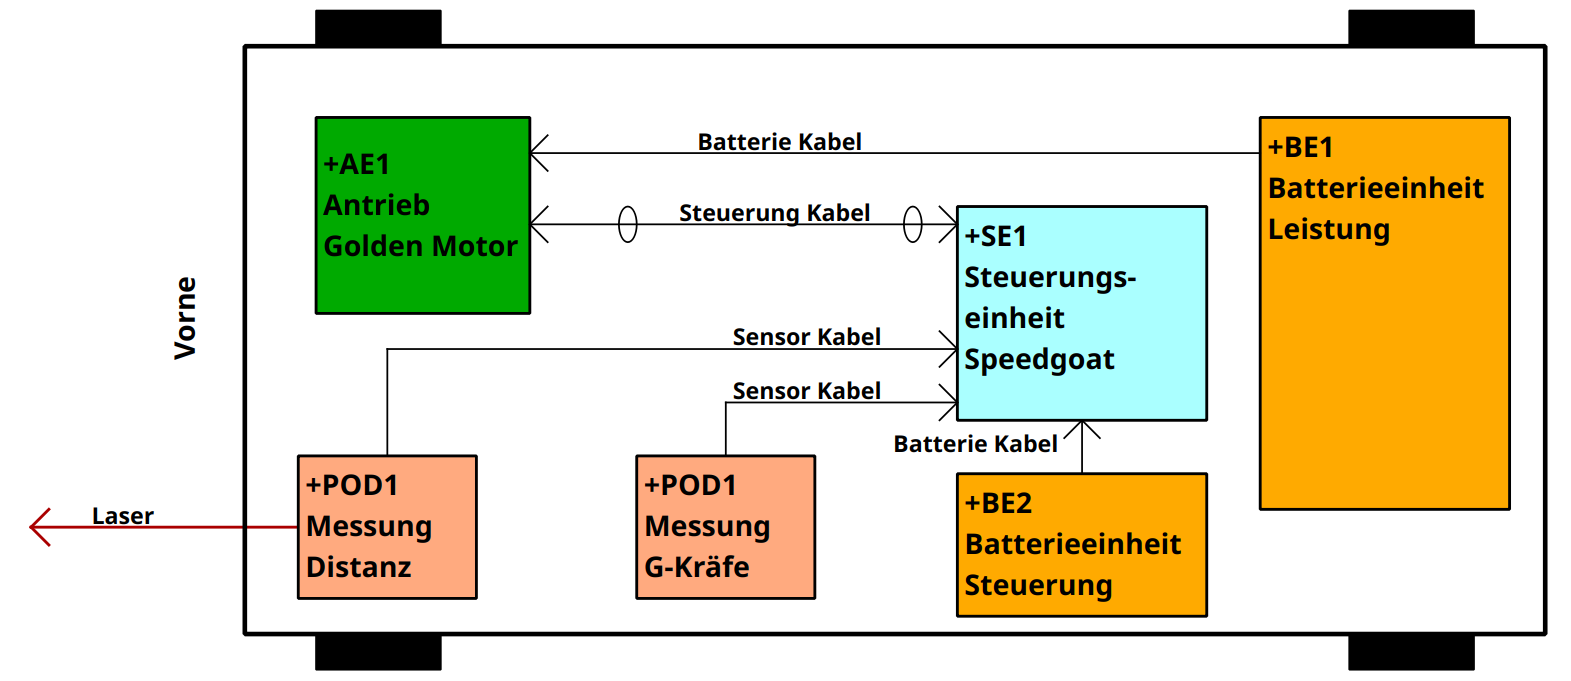
\includegraphics[width=.95\textwidth]{img/3_schaltplan/sp_aufbauplan_0.png}
		\caption{Konzept – Aufbauplan des Fahrzeugs}
		\label{img_1_1:Konzept:0}
	\end{center}
\end{figure}
\pagebreak[1]
Wie in Abbildung \ref{img_1_1:Konzept:0} dargestellt, werden die Baugruppen des Fahrzeugs an verschiedenen Stellen miteinander verbunden. Dabei übernimmt die Steuereinheit (+SE1) eine zentrale Rolle. Mit der echtzeitfähigen Steuerung von Speedgoat werden alle digitalen und analogen Ein- und Ausgangssignale gesteuert, einschließlich der Distanzmessung und der G-Kraft-Messungen. Die Distanzmessung ist für die Positionsermittlung notwendig, während die Beschleunigungskräfte-Messung für Forschungszwecke genutzt werden soll. Die Steuereinheit (+SE1) wird von der Batterieeinheit (+BE2) mit Energie versorgt.\\
Der Antrieb (+AE1) erfolgt über einen BLDC-Motor. Dieser wird mittels eines zusätzlichen Steuergeräts, einem Vector-Controller, angesteuert. Für die Energieversorgung des Antriebs wird eine Leistungsbatterie (+BE1) verwendet.

